\subsection{Příp. užití}

%% Use case - popis, časté použití, příklad

%%%%%%%%%%%%%%%%%%%%%%%%%%%%%%%%%%%%%%%%%%%%%%%%%%%%%%%%%%%%%%%%%%%%%%%%
%% Slide

\begin{frame}{Případy užití}

Diagram případů užití (Use Case Diagram)

\begin{itemize}
	\item Zachycuje způsob, jakým je systém používán
	\item Popisuje funkcionalitu pomocí tzv.
	\begin{itemize}
		\item Účastníků (Actors)
		\begin{itemize}
			\item Představuje spíše roli, než konkrétní osobu
			\item V této roli může být např. i počítačový systém
		\end{itemize}
		\item Případů užití (Use cases)
		\begin{itemize}
			\item Posloupnost akcí, využití systému účastníky
		\end{itemize}
	\end{itemize}
	\item Systém z vnějšího pohledu
	\begin{itemize}
		\item Nejedná se o popis implementace
		\item Tj. co by měl systém poskytovat
		\begin{itemize}
			\item Např. přihlášení, zobrazení výsledků...
		\end{itemize}
		\item Ne, jak by to měl poskytovat
		\begin{itemize}
			\item Přihlašovací údaje se odešlou, zpracuje je nějaká funkce,
			program se dotáže databáze...
		\end{itemize}
	\end{itemize}
\end{itemize}


\end{frame}

%%%%%%%%%%%%%%%%%%%%%%%%%%%%%%%%%%%%%%%%%%%%%%%%%%%%%%%%%%%%%%%%%%%%%%%%
%% Slide

\begin{frame}{Vztahy v případech užití}

Nejběžnější vztahy jsou

\begin{itemize}
	\item Asociace účastník $\to$ případ užití
	\item Generalizace účastníků
	\item Generalizace případů užití
	\item Relace $<<$Include$>>$
	\begin{itemize}
		\item Společný podpřípad se vyčlení
		\item Do jednotlivých případů se \uv{vloží}
		\item Vkládání je povinné, je nedílnou součástí
		\item Sám o sobě může i nemusí mít smysl
	\end{itemize}
	\item Relace $<<$Extend$>>$
	\begin{itemize}
		\item Jeden případ rozšiřuje jiný
		\item Původní případ je kompletní a samostatný
		\item Rozšíření na něj navazuje
		\item Body rozšíření
	\end{itemize}
\end{itemize}	
	
\end{frame}

%%%%%%%%%%%%%%%%%%%%%%%%%%%%%%%%%%%%%%%%%%%%%%%%%%%%%%%%%%%%%%%%%%%%%%%%
%% Slide

\begin{frame}{Příklad}
Jednoduchý bug tracking systém - první náčrt
\begin{figure}
	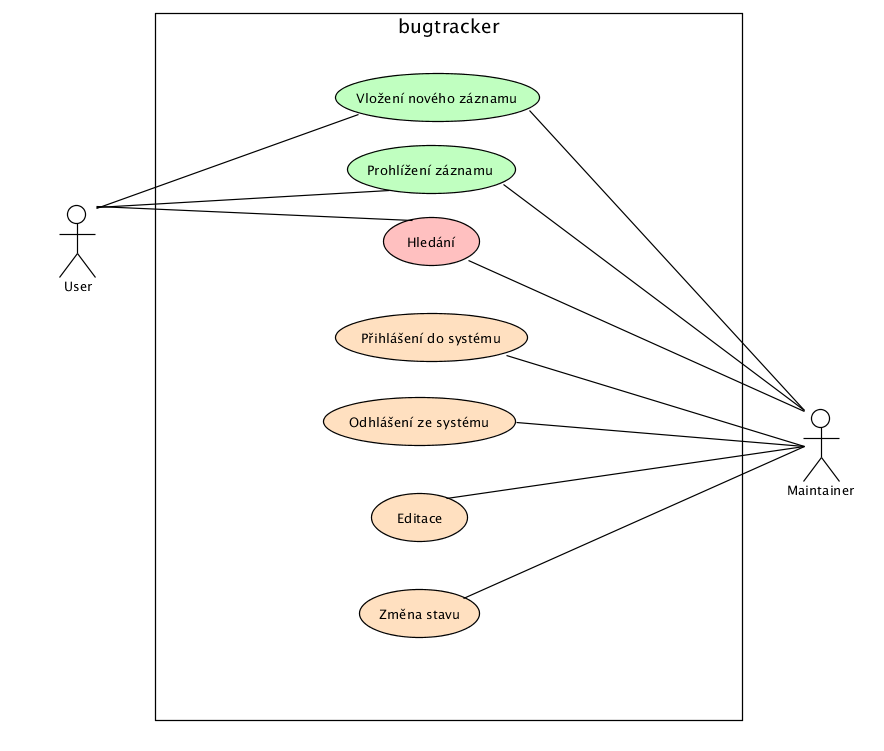
\includegraphics[width=81mm]{img/diagramy/UseCase/bugtracker1.png}
\end{figure}

\end{frame}

%%%%%%%%%%%%%%%%%%%%%%%%%%%%%%%%%%%%%%%%%%%%%%%%%%%%%%%%%%%%%%%%%%%%%%%%
%% Slide

\begin{frame}{Příklad}
Jednoduchý bug tracking systém - generalizace účastníků
\begin{figure}
	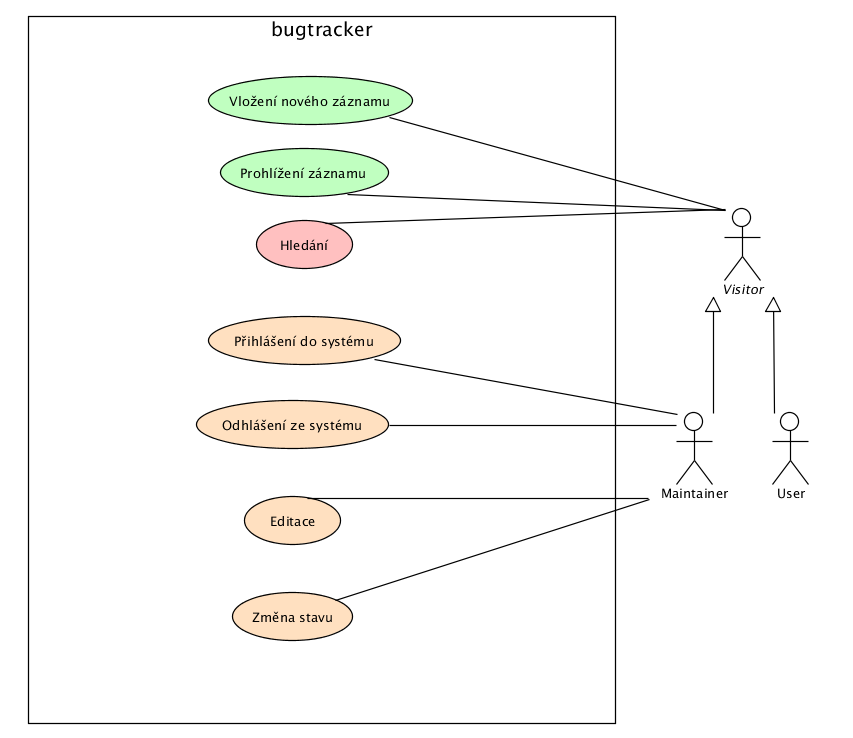
\includegraphics[width=79mm]{img/diagramy/UseCase/bugtracker2.png}
\end{figure}

\end{frame}

%%%%%%%%%%%%%%%%%%%%%%%%%%%%%%%%%%%%%%%%%%%%%%%%%%%%%%%%%%%%%%%%%%%%%%%%
%% Slide

\begin{frame}{Příklad}
Jednoduchý bug tracking systém - finální verze
\begin{figure}
	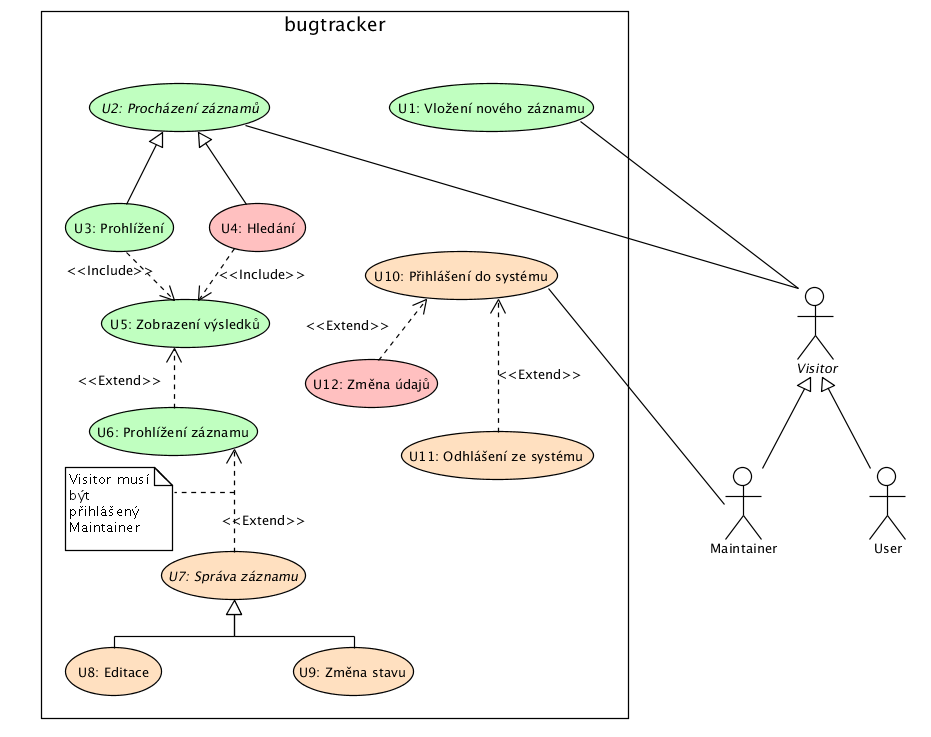
\includegraphics[width=83mm]{img/diagramy/UseCase/bugtracker3.png}
\end{figure}

\end{frame}

%%%%%%%%%%%%%%%%%%%%%%%%%%%%%%%%%%%%%%%%%%%%%%%%%%%%%%%%%%%%%%%%%%%%%%%%
